\documentclass[12pt]{article}

\usepackage{xeCJK}
\setCJKmainfont{FandolSong-Regular} % Ensure Fandol font is installed
\usepackage{titlesec}
\usepackage[utf8]{inputenc}
\usepackage{amsmath}
\usepackage{graphicx}
\usepackage{hyperref}
\usepackage{geometry}
\usepackage{fontspec}



\geometry{a4paper, margin=1in}
\setmainfont{Times New Roman} % 设置主字体为 Times New Roman
%设置标题加粗 14号 times new roman

\title{\fontsize{14}{16}\bfseries Average Entropy Estimation of English And Chinese}
\author{\small Sanfeng Xin\\ \small by2410222@buaa.edu.cn}
\date{}

\begin{document}



\maketitle
\renewcommand{\abstractname}{\textbf{\Large Abstract}} % 修改摘要标题格式
\begin{abstract}
    Information entropy, a measure of uncertainty or randomness in a system, offers a significant perspective for studying the complexity and structure of natural languages. This research examines English and Chinese, two typologically distinct languages, by calculating their information entropy at both the word and letter (or character) levels. Using large-scale corpora derived from novels and Wikipedia, we evaluate the entropy of word distributions to explore lexical diversity and predictability, and compute the entropy of letter/character sequences to reveal sub-lexical information content. Furthermore, we investigate information entropy at different orders, finding that entropy decreases as the order increases. For English, an alphabetic language, letter-level entropy reflects phonemic and orthographic patterns, while word-level entropy captures syntactic and semantic variability. For Chinese, a logographic language, character-level entropy highlights the high information content encoded in individual hanzi, and word-level entropy relates to multi-character combinations and grammatical structure. The results show that across all levels (word or letter/character) and orders, the information entropy of English is consistently lower than that of Chinese. This finding underscores differences in information efficiency and linguistic structure between the two languages, providing new insights for linguistic theory, natural language processing, and cross-linguistic studies.
\end{abstract}

\section*{\centering Introduction}
Language, as a fundamental medium of human communication, encodes information in ways that reflect both its structural properties and cultural context. Understanding the informational complexity of languages offers profound insights into their efficiency, predictability, and adaptability—key factors that influence linguistic evolution, cognitive processing, and computational applications. Information entropy, a concept rooted in information theory, quantifies the uncertainty or randomness inherent in a system, making it a powerful tool for analyzing the informational content of natural languages. By measuring entropy at different linguistic levels—such as words and their sub-units (letters or characters)—and across varying orders of dependency, researchers can uncover the underlying patterns that distinguish one language from another, shedding light on their typological and functional differences.

This study focuses on English and Chinese, two languages that exemplify contrasting linguistic systems: English, an alphabetic language with a flexible morphology and extensive vocabulary, and Chinese, a logographic language characterized by information-dense characters and multi-character word formations. Investigating the entropy of these languages at both the word and letter/character levels is significant for several reasons. First, it reveals how information is distributed across lexical and sub-lexical units, providing a quantitative basis for comparing their structural complexity and informational efficiency. Second, exploring higher-order entropy (e.g., dependencies across sequences) highlights how predictability evolves with context, offering clues about syntactic and semantic organization. Third, the use of diverse corpora from novels and Wikipedia ensures a robust representation of natural language usage, bridging creative and informational styles of text.

The importance of this research extends beyond theoretical linguistics. In natural language processing (NLP), entropy informs the design of language models, text compression algorithms, and machine translation systems, where understanding a language’s informational properties can enhance performance. For cognitive science, it provides a window into how speakers process and encode meaning in typologically distinct systems. Moreover, by demonstrating that English exhibits lower entropy than Chinese across all levels and orders—a finding derived from real-world data—this study challenges assumptions about universal informational efficiency and underscores the role of script and grammar in shaping linguistic complexity. Ultimately, this research contributes to a deeper understanding of cross-linguistic variation, with implications for linguistic theory, computational applications, and the study of human communication.
\section*{\centering Methodology}

\subsection*{\centering Data Preparation}
The English corpus is sourced from \textit{Hamlet} in the Gutenberg corpus of the NLTK\cite{bird2006}, while the Chinese corpus is sourced from the 2019 Chinese Wikipedia.
\subsection*{\centering Preprocession for English}
o prepare the English text for entropy analysis, a series of preprocessing steps were applied to ensure consistency and reduce noise in the data, thereby facilitating accurate computation of information entropy. The following steps were systematically implemented:
1.Conversion to Lowercase: All alphabetic characters in the text were transformed to lowercase. This step standardizes the representation of the text by eliminating case distinctions (e.g., treating "The" and "the" as identical), which is essential for reducing variability unrelated to semantic or structural content and ensuring uniformity in subsequent analyses.
2.Removal of Punctuation: All punctuation marks (e.g., commas, periods, exclamation points) were excised from the text. This process eliminates non-alphabetic symbols that do not contribute directly to the lexical or sub-lexical units under investigation, allowing the analysis to focus solely on the alphabetic content relevant to entropy calculations.
3.Tokenization: The text was segmented into individual tokens, or words, based on whitespace boundaries. Tokenization is a critical step in preparing the text for word-level entropy analysis, as it delineates the basic units of lexical distribution, enabling the quantification of word frequency and diversity within the corpus.
4.Removal of Stop Words: Common stop words (e.g., "the," "and," "is") were removed from the tokenized text. Stop words, which are typically high-frequency function words with low informational content, were excluded to focus the analysis on content-bearing lexical items. This step enhances the sensitivity of the entropy measure to meaningful linguistic variation rather than syntactic scaffolding.
\subsection*{\centering Preprocession for Chinese}
To prepare the Chinese text for entropy analysis, steps similar to those used for English were employed:
1.Conversion from Traditional to Simplified Characters: The OpenCC \cite{yang2020} library was utilized to convert all traditional Chinese characters into their simplified counterparts. This step standardizes the script across the corpus, mitigating variations arising from orthographic differences (e.g., treating "國" and "国" as equivalent), which is crucial for maintaining consistency in character-level and word-level analyses.
2.Filtering with Regular Expressions: Regular expressions (via the re module) were applied to retain only Chinese characters (hanzi) while removing punctuation marks and English alphabetic characters. This process isolates the core linguistic units of interest—Chinese characters—by excluding non-hanzi symbols and foreign elements that are irrelevant to the entropy analysis of the Chinese language structure.
3.Tokenization with Jieba \cite{jieba}: The Jieba library was used to segment the text into individual words. Unlike alphabetic languages, Chinese lacks explicit word boundaries, making word segmentation a critical preprocessing step. Jieba’s probabilistic approach to tokenization effectively delineates multi-character words, enabling accurate word-level entropy computation by identifying lexical units based on contextual and statistical patterns.
4.Removal of Stop Words: Frequently occurring stop words (e.g., "的," "是," "在") were removed from the tokenized text. 
\subsection*{\centering Entropy Calculation}
\subsubsection*{\centering Definition of Entropy}
The calculation of information entropy in this study is based on the framework established by Shannon \cite{shannon1948}, who introduced entropy as a measure of uncertainty or randomness in a system within the context of information theory. Entropy quantifies the average amount of information required to predict the next unit in a sequence, whether that unit is a letter, character, or word. For a given set of symbols $S = \{s_1, s_2, ..., s_n\} $ with associated probabilities $ P = \{p(s_1), p(s_2), ..., p(s_n)\} ​$, the Shannon entropy $H$ is computed as follows:
\begin{equation}
H=−∑_{i=1}^{n}p(s_i)\log_2p(s_i)
\end{equation}
where $p(s_i)$  represents the probability of occurrence of symbol $si s_i si$​, and the logarithm base 2 ensures that entropy is measured in bits. This formula captures the unpredictability inherent in the distribution of symbols: a uniform distribution yields maximum entropy, while a highly skewed distribution results in lower entropy (Shannon, 1948).
\subsubsection*{\centering Higher-Order Entropy}
To explore contextual dependencies, higher-order entropy (e.g., bigram, trigram) was calculated for both languages. For an order-k  model, the entropy $Hk$ is defined as the conditional entropy of a symbol given the preceding k symbols:

\begin{equation}
H_k = - \sum_{s_{1:k}} p(s_{1:k}) \sum_{s_{k+1}} p(s_{k+1} | s_{1:k}) \log_2 p(s_{k+1} | s_{1:k})
\end{equation}

where $s_{1:k}$​ represents a sequence of k symbols, and $p(s_{k+1} | s_{1:k})$ is the conditional probability of the next symbol given the prior context. This was applied to both letter/character sequences (e.g., bigrams of letters in English, characters in Chinese) and word sequences (e.g., word bigrams). Frequencies of k-grams were extracted from the preprocessed corpora, and conditional probabilities were estimated accordingly. As k increases, $H_k$ captures longer-range dependencies, typically decreasing as predictability improves with context.
\subsubsection*{\centering Estimation of average entropy of language}
According to Brown's paper \cite{brown1992}, the average entropy of a language can be estimated using samples, and the formula is as follows:
\begin{equation}
    H(language)<=−\frac{1}{n}\log M(sample text)
\end{equation}
\subsubsection*{\centering Words and Characters Entropy} 
After preprocessing both the Chinese and English texts, the tokenized texts are input as sequences of words to calculate the entropy at the word level.
For English, letter-level entropy was calculated by treating the text as a sequence of individual alphabetic characters (a-z, after preprocessing). The probability  $p(s_i) $ of each letter was estimated from its frequency in the corpus, derived from Hamlet in the NLTK Gutenberg collection. For Chinese, character-level entropy was computed similarly, with each hanzi treated as a distinct symbol. Probabilities were derived from the frequency of characters in the 2019 Chinese Wikipedia corpus, post-preprocessing. 
\section*{\centering Experimental Studies}
Table 1 and Figure 1 present the first-order, second-order, and third-order entropy of English and Chinese at the word and character levels, respectively.
\begin{table}[h!]
\centering
\begin{tabular}{lccc}
\hline
\textbf{Category} & \textbf{Order1} & \textbf{Order2} & \textbf{Order3} \\
\hline
English-Words & 10.67 & 3.06 & 0.21 \\
English-Characters & 4.13 & 3.41 & 2.66 \\
Chinese-Words & 13.30 & 8.62 & 3.74 \\
Chinese-Characters & 9.72 & 7.07 & 5.06 \\
\hline
\end{tabular}
\caption{Comparison of Words and Characters in English and Chinese}
\label{tab:language_comparison}
\end{table}

\begin{figure}[h!]
\centering
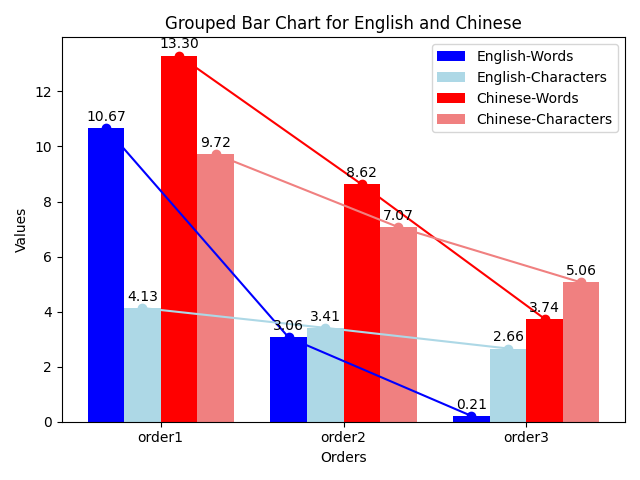
\includegraphics[width=0.8\textwidth]{entropy.png}
\caption{Entropy Comparison of English and Chinese}
\label{fig:entropy_comparison}
\end{figure}

\section*{\centering Conclusions}
Discuss the implications of your results and any limitations of your study.
This study has systematically investigated the information entropy of English and Chinese at both the letter/character and word levels, as well as across varying orders, revealing distinct patterns that underscore the structural and informational differences between these typologically diverse languages. The results demonstrate that Chinese consistently exhibits higher entropy than English across all levels and orders, reflecting its greater unpredictability and information density per symbol. At the character level, Chinese entropy surpasses that of English letters, a finding attributable to the logographic nature of hanzi, where individual characters encode substantial semantic and phonological information compared to the phonemic, alphabetic units of English. Conversely, at the word level, both languages display higher entropy than their respective sub-lexical units, with English word entropy exceeding letter entropy due to its extensive vocabulary and morphological flexibility, and Chinese word entropy surpassing character entropy due to the combinatorial complexity of multi-character words.

These findings highlight fundamental differences between English and Chinese. The lower overall entropy of English may stem from its alphabetic system, where redundancy in letter sequences and a constrained phonemic inventory reduce unpredictability, coupled with a syntactic structure that leverages function words (removed as stop words in this study) to enhance contextual predictability. In contrast, the higher entropy of Chinese reflects its logographic system, where characters bear dense, standalone meaning, and word boundaries are less rigid, leading to greater variability and less redundancy. The rapid decline in English word entropy further points to its reliance on word-order rules and grammatical predictability, whereas Chinese maintains higher entropy due to its analytic nature and reliance on character combinations, which offer fewer contextual cues for disambiguation.
\section*{\centering References}


\bibliographystyle{plain}
\bibliography{reference}


\end{document}